% !TEX root =  paper.tex
\section{Approach}

In this chapter, we propose an approach to
automatically test for a subset of web accessibility violations 
that are pertinent to semantic structure.
We recall that the scope of this work focuses on  
vision disabilities as opposed to other forms of disability, 
due to the web being a predominantly visual medium 
and the fact that vision disabilities 
are the most common software-related disability~\cite{2019users_survey}. 

\Cref{fig:approach} shows an overview of our 
proposed approach, which is based on the strategy of visually 
analyzing the web page to infer semantic groupings and their roles, 
and then checking that the HTML markup matches the inferred semantic roles.
The approach begins by obtaining the Document Object Model (DOM)
and screenshot of the web page rendered in a web browser.
Next, the set of visibly perceivable objects is identified.  
This is then used to perform a semantic grouping of the page into 
a set of semantically coherent regions. 
Subsequently, this information is used in an 
inference stage where the specific semantic role 
of each region is detected.
Finally, the inferred semantics are checked against the markup
used in the page, and a report is generated as to which 
parts of the page are inaccessible.
The rationale behind this strategy is to check whether 
  the semantics visually perceivable by sighted 
users are reflected in the semantics of the HTML markup,
thereby ensuring accessibility. 

\begin{figure}[t]
    \centering
    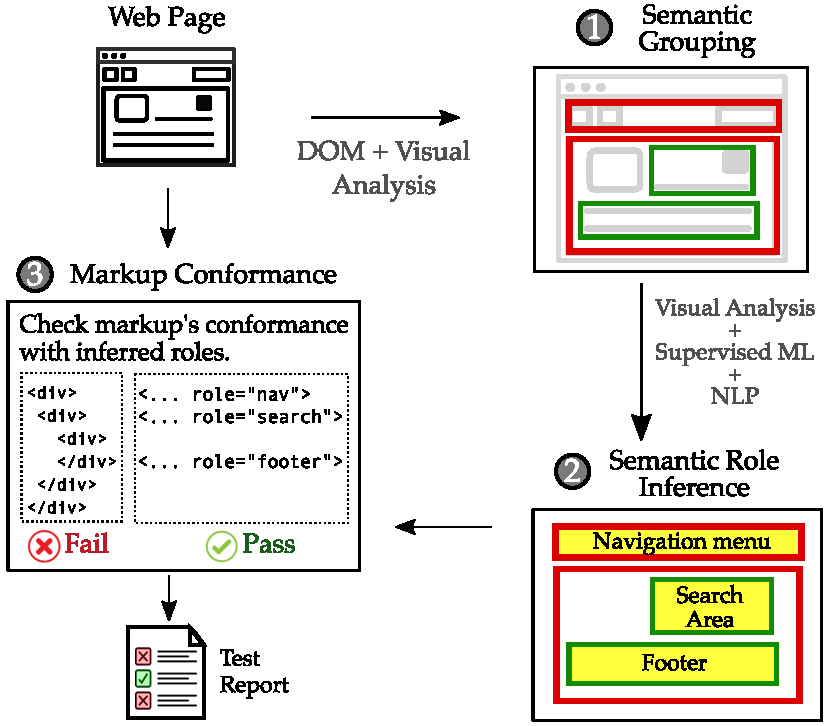
\includegraphics[width=0.7\linewidth]{accessibility_testing/figures/approach/approach.pdf}
    \caption{Overview of the proposed approach.}
    \label{fig:approach}
\end{figure}

\subsection{Visual Objects Identification}
In this first stage,
the goal is to identify objects that 
are perceivable by sighted users, which we refer to as \emph{\vizobjs}. 
For instance, in \Cref{fig:motivating-example}(c), 
each item in the top navigation menu would be a {\vizobj}. 
This step of visual objects identification is the 
foundation of our overall approach, 
since the identification of {\vizobjs} enables checking whether the information
and elements that are perceivable by sighted users 
are also accessible to non-sighted users. 
 

\subsubsection{Objects Extraction}\label{subsec:extraction}

We begin by taking as input the DOM of the page 
after it is loaded and rendered in a browser. We 
then extract from the DOM a set of nodes that 
represent visual content of the page, 
and we refer to each of these as \emph{{\VizObjs}}.
We define three types of {\VizObjs}:
textual, image, and interactive.

\header{Textual Objects}
The extraction of text content is achieved by 
traversing text nodes of the DOM. More specifically:
\begin{align}
    \Theta_{t} \coloneqq \{ E \:\vert\: \nu(E) \land \tau(E) \}
\end{align}
where $\Theta_{t}$ is the set of all {\vizobjs} that represent text in the page,
$E \in DOM$ is a leaf element iterator of the rendered DOM in the browser,
$\nu(E)$ is a heuristic predicate that runs a series of checks
to detect visually perceivable elements (as will be described in \cref{subsub:vizassert}),
and $\tau(E)$ is a predicate that examines whether
there is a text associated with $E$. 
More specifically, it returns
non-empty nodes of DOM type \code{\#TEXT},
which represent string literals. 
An example of extracted textual objects would be the ``Resources'' section in 
\Cref{fig:motivating-example}(c).
We note that the predicate is based on a node type, rather than
an element (i.e., tag) type.
This allows more robust abstraction because the predicate captures any text and does not
make assumptions about how developers choose to place their text.
In other words, regardless of the tag used for text data (e.g., \code{<span>, <div>}),
text would still be stored in nodes of type \code{\#TEXT}, even for custom HTML elements.
This helps in making the approach more robust by reducing assumptions about
tags and how they are used in the page.

\header{Image Objects}
Subsequently, we perform another extraction for image objects.
We define this as follows:
\begin{align}
    \Theta_{m} \coloneqq \{ E \:\vert\: \nu(E) \land \mu(E) \}
\end{align}
where $\Theta_{m}$ is the set of all objects that are present in the page and represent images.
As in the previous case,
the predicate $\mu(E)$ examines whether
there is any relevant image content associated with $E$.
This has two possibilities:
a) nodes of \code{<img>}, \code{<svg>}, and \code{<canvas>} elements, 
and b) non-image nodes with a non-null background image.
An example of extracted image objects would be the bell icon in 
\Cref{fig:motivating-example}(c).
We note that this predicate makes the proposed approach more robust
by eliminating assumptions about how developers markup images. 
If images are contained in standard tags (e.g., \code{<img>}, \code{<svg>}),
then the predicate readily captures them. 
However, we make no assumptions that this is the only way an image can be included.
For this reason, we also capture elements of any type when a non-null background image 
is detected.

\header{Interaction Objects}
Finally, we extract the interaction elements as follows:
\begin{align}
    \Theta_{i} \coloneqq \{ E \:\vert\: \nu(E) \land \eta(E) \}
\end{align}
where $\Theta_{i}$ is the set of all {\vizobjs} that represent form elements 
or similar interactive elements.
These are determined by the predicate $\eta(E)$, which collects
elements such as input fields and drop down menus.
An example of extracted interaction objects would be the Email 
input field in \Cref{fig:motivating-example}(c).


\subsubsection{Visual Assertion}\label{subsub:vizassert}
After the preceding extraction of an initial set of {\vizobjs}, 
this stage proceeds by conducting a visual analysis of the objects. 
This analysis detects if an object is visually perceivable.
We conduct the visual analysis as follows. First, we obtain the box model of 
each object. We use the \emph{computed} box model in order to faithfully 
capture the location as finally rendered on screen. 
Next, we obtain a screenshot of the region defined by the box model. 
We then analyze the screenshot using the Prewitt operator~\cite{nixon2019feature} 
used in computer vision. This operator applies a set of derivatives or 
differentiation operations on the image, and then typically used to detect 
salient visual features in the image (e.g., shapes, textures). 
We therefore use this operator to extract any visual features present in the image,
regardless of the category or form of these features. 
Depending on the presence or absence of visual features in the image, the perceptibility state of the object is determined.
If no visual features are detected, 
the object is deemed to be non-perceivable, and vice versa. 
For example, consider \Cref{fig:motivating-example}(c).
The navigation region in the top, and the 
main content that follows it, are perceivable by sighted users. 
However, web pages also have spacing elements that 
do affect the layout but are not individually perceivable themselves. 
For instance, there can be an element between the navigation bar 
and the ``Resources'' section such that a certain vertical distance is 
maintained below the navigation bar. While such a spacing element certainly 
affects the layout and occupies screen space, 
it does not constitute a {\vizobj} due to it's imperceptibility. 

\subsection{Semantic Grouping} \label{sec:grouping}

After the {\vizobjs} identification is completed,
we proceed by grouping {\vizobjs} into groups representing potential
semantically relevant regions on the page. 
For instance, in \Cref{fig:motivating-example}(c), 
one semantic grouping would be the navigation region 
at the top of the page. 
Another semantic grouping would be the ``Resources'' and ``About Us'' 
sections representing the main content of the page.

The rationale for this step of the approach is as follows. 
We recall that screen readers expect the markup to indicate the 
major semantic regions of a page. 
Accordingly, in order to automatically assert that any visually perceivable semantic 
region has been also expressed in the markup, we first need 
a mechanism by which we can detect the semantic regions in the first place. 
This is what we aim to achieve in this stage. 
Here we are only concerned with creating potential semantic groupings, 
while the next stage (\Cref{sec:role-inf}) attempts to infer what is the semantic 
role (if any) of each potential grouping. 

\hl{
The grouping uses both structural (DOM) information as well as visual analysis. 
The DOM is used to generate a large number of potential seed groupings, 
and the visual analysis performs filtering and further analysis to produce a 
final set of groups.
We adopted this strategy for the following reasons. 
We observed that the DOM can potentially serve as a source of seed groupings. 
This is because of its inherently hierarchical nature that also tend to capture 
the developer's or designer's own intended semantic grouping.
That is, the assumption here is that a set of nodes that has been grouped by a developer 
(i.e., implicitly via DOM hierarchy) is more \emph{potentially} likely to represent some 
semantic value, compared to a random set of nodes. 
We emphasize that the groups only potentially have semantic value, and therefore serve 
only as an initial guess. The final decision 
of whether or not they do actually have a semantic role will be determined at a later stage (i.e., the role inference stage). 
Had we not performed this initial guess, the role inference alone would be practically 
untenable because of the extremely large combinatorial set of possible node combinations. 
}
Subsequently, visual analysis filters these initial seed groups and process 
them to construct semantic groupings. 
Visual analysis is used because, while the DOM may provide seed groupings, 
it does not faithfully represent what the end user is actually observing on the screen. 


\header{Grouping process}
We now describe the mechanism of the grouping process.
First, we obtain one flat non-hierarchical set of all DOM elements. 
For instance, in \Cref{fig:motivating-example}(a), 
this would be all the \code{div} elements in one flat set.
The elements are collected regardless of visibility, due to the complex 
nature of DOM and CSS rendering where non-visible nodes can contain visible children.
For this same reason, the initial set of elements is flat and non-hierarchical, 
because visible children can often be inside non-visible nodes, and therefore relying 
on DOM hierarchy would yield many false positives and negatives. 
Instead, we build the hierarchy by visually analyzing the collected flat set of elements.
We do this by first collecting the computed box model of each element in the set. 
For instance, in \Cref{fig:motivating-example}(a), this would result in a set containing 
the computed box model of each \code{div} element regardless of hierarchy.
Next, we remove box models that are visually located outside the page boundaries, 
since they are not perceivable to sighted users.
For boxes that are only partially outside the page, we trim them to page boundaries. We note that we analyze the page as a whole, 
not only the currently visible portion. 
Subsequently, we filter \emph{equivalent} boxes, which is when a pair of boxes 
visually contain the same set of {\vizobjs}.
We do this by removing the smaller box in terms of visible area in a pair of equivalent boxes. This is because multiple boxes will often 
exist since many DOM elements can share similar visual dimensions 
and regions on screen. 
Next, we filter boxes based on how many {\vizobjs} are visually contained (i.e., located) 
within them. We remove each box that visually contains the entire set of {\vizobjs} on the page. 
For instance, in \Cref{fig:motivating-example}(a), any \code{div} that 
visually contains the entire set of all \code{div}s is removed.
This is because such a set does not represent any semantically useful grouping, 
since the entire set of objects is in one group only. 
Finally, we iterate over the set of {\vizobjs}. 
For each object, we find the largest box that visually contains the object. 
Once this is completed for all {\vizobjs}, the final result is a set of boxes representing 
the potential semantic groupings on the page.


\subsection{Semantic Role Inference}\label{sec:role-inf}
Once semantic grouping is completed, we proceed to infer 
the semantic role of each group. 
This step infers one of the pre-defined landmark roles (\Cref{subsec:aria-roles}). 
An example can be seen in the top navigation bar in \Cref{fig:motivating-example}(c), 
indicating the pre-defined role of \code{navigation}. 
However, not all roles are relevant to our scope of automated 
semantic analysis. For instance, \code{region} is a generic catch-all label that 
does not convey any specific semantic role, and its use is generally discouraged 
and typically not used by screen readers. 
Another example is \code{form}, a label that indicates form regions. 
The label is directly associated with HTML \code{<form>} elements, 
and therefore no semantic analysis or inference is needed for its detection.
Accordingly, we focus our semantic analysis on the more relevant roles of 
\code{main}, \code{navigation}, \code{contentinfo}, and \code{search}, 
which will be described in the following sections. 


\header{Main Role}
The \code{main} ARIA role indicates a region that contains the main output or results 
in a web page. For example, on the search results page of a search engine, 
the region containing the list of retrieved search results would be the main region, 
which is then surrounded by other regions such as the navigation bar or footer.

The process by which we infer the role of a group to be \code{main} is as follows.
First, we compute a score for each detected group in the page. 
The score uses both visual geometrical attributes as well as natural language 
processing (NLP) measurements.
More specifically: 
\begin{align} \label{eqn:score_main}
    \psi_{main}(r) = A(r) \rho(r)
\end{align}
where $r$ is a semantic grouping of the page, $\psi_{main}$ is the score, 
$A(r)$ is the visual geometric area for $r$, and $\rho(r)$ is an NLP 
metric we define to measure linguistic aspects of the contents of $r$. 
More specifically, $\rho(r)$ 
first performs a part-of-speech (POS) tagging, which is a common NLP analysis 
than assigns POS labels (e.g., verb, noun, adjective) to each word. 
$\rho(r)$ then measures the variance of the linguistic POS tag frequencies 
of all textual objects contained in $r$.  
We give an example to clarify the various measured values. 
Consider the rendered page in \Cref{fig:motivating-example}-c. 
$r$ would represent, for instance, the region containing the 
body of the page (e.g., the Resources and About Us sections). 
$A(r)$ would be the geometric area of that region as visible on the screen. 
The rationale is to capture how much would a region occupy the 
visible space for sighted users. 
As for $\rho(r)$, it first collects all textual objects 
(as explained in \cref{subsec:extraction}) within $r$, which would 
collect all text elements such as "Resources", "About Us", as well as the 
paragraphs on the page. For each text object, POS tags are collected,  
and then their frequencies (i.e., count of each tag type) are computed. 
$\rho$ then measures the variance of these POS tag frequencies. 
For instance, a navigation region $r$ that has, say, the textual objects ``Images'', 
``News'', and ``Settings'' has no variance since they all 
have identical POS tags. Contrast this with the main body of text in a page, 
which contains elements such as such as paragraphs, 
section headings, links, and much more. The likelihood of all such content 
to be linguistically monotonous (i.e., all tags are nouns) is practically negligible.
This is why \cref{eqn:score_main} includes the $\rho(r)$ factor.
The $A(r)$ in the equation accounts for the fact that it is unlikely that the main 
region of the page would be the visually smallest area on the page. 
Once the score in \cref{eqn:score_main} is computed for all detected regions, 
we sort the regions by score and select the region with the highest score, 
which is finally reported to be the region having the main role. 
We note that we simply directly multiply the two factors, and do not have any thresholds or weights in order to have a parameter-free and more robust inference. 

\header{Navigation Role}
The \code{navigation} ARIA role indicates a region in a webpage that 
allows users to navigate between various pages or views. 
The process by which we infer the role of a group to be \code{navigation}
is as follows. 
We first compute a score for each group, using the 
following equation:
\begin{align} \label{eqn:score_nav}
    \psi_{nav}(r) = \frac{C(r)}{1 - \rho_h(r)} 
\end{align}
where $r$ is a semantic group of the page, $\psi_{nav}$ is the score, 
and $C(r)$ is a metric that measures the \emph{clickables ratio} 
inside the group $r$. This computes the ratio of {\vizobjs} 
that appear to be clickable to sighted users, which we define as 
any {\vizobj} whose onscreen cursor is a hand or a pointer, 
indicating to sighted users that it can be clicked on. 
Accordingly, a group that has high $C(r)$ is mostly composed 
of objects that a sighted user can click on, which is typically the case 
for navigation regions. 
For example, in \Cref{fig:motivating-example}-c, the yellow 
navigation region at the top contains elements that all appear 
as clickables to sighted users. 
In contrast, a group that does not contain any clickables 
(e.g., only static texts and images) would have a $C(r)$ equal to zero and 
therefore is not a navigation region. 
This can be seen, for instance, in \Cref{fig:motivating-example}-c 
in the body of the page below the navigation bar, where the body 
contains only static text paragraphs or images. 
$\rho_h(r)$ is a measure of the homogeneity of the contents of $r$. 
For semantic groups containing only textual elements, 
$\rho_h(r)$ is the same NLP linguistic 
variance metric we defined in \cref{eqn:score_main}. 
For all other elements, $\rho_h(r)$ represents the dimensional variance 
of the objects in $r$.
Finally, a given group is inferred to have a navigation role 
when $\psi_{nav}$ greater than or equal unity, which was determined experimentally by manually testing this value empirically on a random group of websites.


\header{ContentInfo/Footer Role}
The \code{contentinfo} role (also known as the footer role) indicates 
regions of the page that represent complementary 
content to the parent document. That is, instead of containing the 
main output of the page or the main navigation elements, footer regions 
serve as complementary content or information that comes after 
the main content. 
In a similar fashion to previous roles, we compute a score for each detected 
grouping, using the following equation:
\begin{align} \label{eqn:score_footer}
    \psi_{footer}(r) = \frac{C(r)D(r)}{A(r)} 
\end{align}
where, as in the previous roles, $r$ is a semantic group of the page, 
$\psi_{footer}$ is the score, 
$A(r)$ is the visual pixel count for $r$, $D(r)$ is the visual 
distance from the geometric center of $r$ to the origin of the screen, 
and $C(r)$ is the clickables ratio in $r$ as defined in \cref{eqn:score_nav}.
As can be observed from the equation, the score is mostly concerned 
with the visual geometric aspects of the region, since this ARIA role
is, by definition, spatial in nature since it refers to a specific 
spatial visual placement on the page. 
Accordingly, we compute and sort the score for all groups, 
and select the group with the highest score. If the group is located 
in the lower half of the page, it is reported as a footer. Otherwise no 
footer regions are reported.

\header{Search Role}
The \code{search} ARIA role indicates regions in a page 
that allow users to enter a search query and retrieve items on 
the page or site. To infer this role, we use a combination of 
visual analysis, a supervised machine learning model, as well as 
linguistic (i.e., keyword) techniques.

First, we train a Convolutional Neural Network (CNN) to visually 
recognize search icons. We collected and labeled 
500 data points representing icon images (50\% positive examples) 
and used the Inception CNN architecture~\cite{szegedy2015rethinking}, 
which has been shown to produce very effective classifications for 
computer vision machine learning problems~\cite{szegedy2015rethinking}.
Subsequently, we use this model to find search icons on a page. 
Next, we perform a nearest neighbor search to look for text input 
fields in the spatial vicinity of detected search icons. If a text input field 
is found, we mark the region containing the search icon and the input field 
as having a search semantic role.
Furthermore, we also check for cases where the search input text field 
has no associated search icons. In this scenario, we extract all text 
input fields on the page. We then perform a nearest neighbor search 
to find any visible label texts in the visual spatial vicinity around 
the input field.
We then conduct NLP \emph{stemming} on the label text and find those that 
include key linguistically significant \emph{stem words},
such as ``find'', ``search'', and ``locate.'' 
Any detected group that matches any of the above cases is marked 
as having a search semantic role.

Finally, we note that, due to the non-hierarchical nature of our semantic groupings, 
all inferred roles are agnostic to hierarchies and the proposed approach is therefore able to detect hierarchical combinations of the inferred roles (e.g., a navigation region within a footer region). 



\subsection{Markup Conformance}\label{sec:conformance}
This final stage asserts that the source of the page 
contains markup indicating the presence of the inferred semantic regions
and their semantic roles. 
For instance, in \Cref{fig:motivating-example}(c), the approach so far 
would infer that the group of elements at the top of the page represent 
a coherent semantic grouping, and that their semantic role is navigation.
If the HTML markup corresponding to that area does not contain 
the ARIA landmark role of \code{navigation}, 
then screen readers will not be able to provide this semantic information 
to users, and we recall that this semantic information is 
among the most important and widely used of ARIA roles by users 
with disabilities~\cite{2019users_survey}. 
Therefore, in such cases where the markup does not 
conform to the inferred 
semantic roles, we report an accessibility failure 
and indicate the expected 
semantic markup and where it should have been 
expressed in the page.

The mechanism of checking markup conformance is as follows. 
First, we obtain the semantic groupings and any inferred roles, 
as described in the previous sections. 
For each semantic group, we identify all DOM elements that satisfy two criteria:
1) all {\vizobjs} of the group are located inside the element's box model, and 
2) the element's box model is located inside the group's box model.
This process captures all possible DOM elements that would qualify as 
a root for the region, without including objects from other regions. 
Any of these DOM elements would therefore have to contain markup 
indicating the presence of a region and its role.

We then check whether any element in the set meets both of the following requirements: 
1) the element has a \code{role} attribute whose value matches the inferred semantic role of the group.
2) the element's computed box model visually overlaps the box model of the inferred semantic group.
The rationale for adopting this approach is as follows. 
As we noted in \Cref{sec:grouping}, the complex nature of 
DOM and CSS rendering easily allows cases where non-visible/non-rendered 
nodes can contain visible rendered children. A DOM-based approach 
(e.g., checking containment by XPath) would therefore yield many false positives and negatives. 
Accordingly, we use the visual check above for a more robust analysis. 

If an element satisfying these requirements is found, we log it and move on to the next inferred semantic role and check that it has been correctly expressed in the markup. The process is repeated for all semantic groupings for which a role has been inferred. Any semantic grouping for which no role has been inferred is discarded. A report is finally generated indicating all roles that have been correctly expressed in markup, and all roles that should have been 
in the markup but are missing. We do not assume our approach understands the semantic roles better than what a human being would manually identify, and therefore there no miss-classification is reported if a markup already exists.  

\header{Implementation}
We implemented the proposed approach in a tool called~\toolname  
(short for Accessibility Ray). It is implemented in Java. 
We use Selenium WebDriver to instrument browsers and extract 
DOM information and computed attributes. We use OpenCV~\cite{opencv} 
for computer vision computations, DeepLearning4J~\cite{dl4j} for machine learning operations, and the Stanford CoreNLP library~\cite{stanfordCoreNLP} for linguistic analysis. 
To make the study replicable, we made available online a link to 
our \toolname tool and the anonymized participants' responses~\cite{tool-and-data}.